\documentclass{article}
\usepackage{graphicx} % Required for inserting images
\usepackage{tikz}
\usepackage{algorithm}
\usepackage{algorithmic}
\usepackage{amsmath}
\usepackage{natbib}
\usepackage{booktabs}
\usetikzlibrary{shapes.geometric, arrows}
\newtheorem{teorema}{Teorema}
\title{Análisis de una distribución normal}
\author{José Adrián Rodríguez González }
\date{Septiembre 2024}

\tikzstyle{startstop} = [rectangle, rounded corners, minimum width=2cm, minimum height=1cm,text centered, draw=black, fill=red!30]
\tikzstyle{process} = [rectangle, minimum width=2cm, minimum height=0.5cm, text centered, draw=black, fill=orange!30]
\tikzstyle{decision} = [diamond, minimum width=0.5cm, minimum height=0.1cm, text centered, draw=black, fill=green!30, font=\scriptsize]
\tikzstyle{arrow} = [thick,->,>=stealth]
\begin{document}

\maketitle

\section{Introducción}
El problema se menciona de la siguiente forma de decision:
Una fábrica tiene un proceso que sigue una distribución normal. El tiempo de fabricación de cada pieza sigue depende de varios factores, sin embargo se sabe que de media sigue una media de 30 minutos y una desviación de 5 minutos.
La fábrica posee tres rangos de tiempos.
\begin{itemize}
    \item Los procesos rápidos son aquellos que las piezas tardan menos de 25 minutos
    \item Los procesos medios son aquellos que las piezas tardan entre 25 minutos y 35 minutos
    \item Los procesos lentos son a aquellas piezas que tardan más de 35 minutos
\end{itemize}
De esta forma, se necesita encontrar la suma promedio de cada un de los procesos además de la suma promedio total de cada uno de los procesos.

\section{Objetivos}
\subsection{Objetivo general}
El objetivo general es analizar un conjunto de datos $X$ de producción de piezas, de tal forma que ayude a la empresa a encontrar una mejor estrategia de como debe de gestionar su producción.
\subsection{objetivos específicos}
Para poder llegar al objetivo general, es necesario separar y entender el problema, desde la definición de una distribución normal, como simularla y poder hacer los cálculos adecuados de cada una de las secciones para poder determinar la mejor estrategia para la empresa. 
\section{Procedimiento}
Para comenzar a atacar el problema se necesita comprender el significado de una distribución normal.
Dentro de la gran gama de distribuciones de probabilidad que existen; la distribución normal es la más común y que muchos modelos predictivos utilizan como base.
¿Pero que es una distribución normal?
Se define como 
\begin{equation}
    PDF(x)=\frac{1}{\sigma\sqrt{2\cdot\pi}}e^{-\frac{(x-\mu)^2}{2\sigma^2}}
\end{equation}
Siendo $\sigma$ la desviación y $\mu$ la media. 
\begin{teorema}
    \begin{equation}
        \frac{1}{\sigma\sqrt{2\cdot\pi}}\int_{-\infty}^{\infty}e^{-\frac{(x-\mu)^2}{2\sigma^2}} dx=1
    \end{equation}
\end{teorema}
Con estas definiciones, podemos inferir que la distribución toma en $x$ todo los valores de los números reales. Otra cuestión por la que la distribución normal es muy característica es debido a que la gran mayoría de fenómenos en la naturaleza se describen a traves de esta distribución. Por loq ue la distribución de tiempos en la producción de piezas es una de ellas.
\subsection{Diagrama de datos}
\scalebox{0.8}{
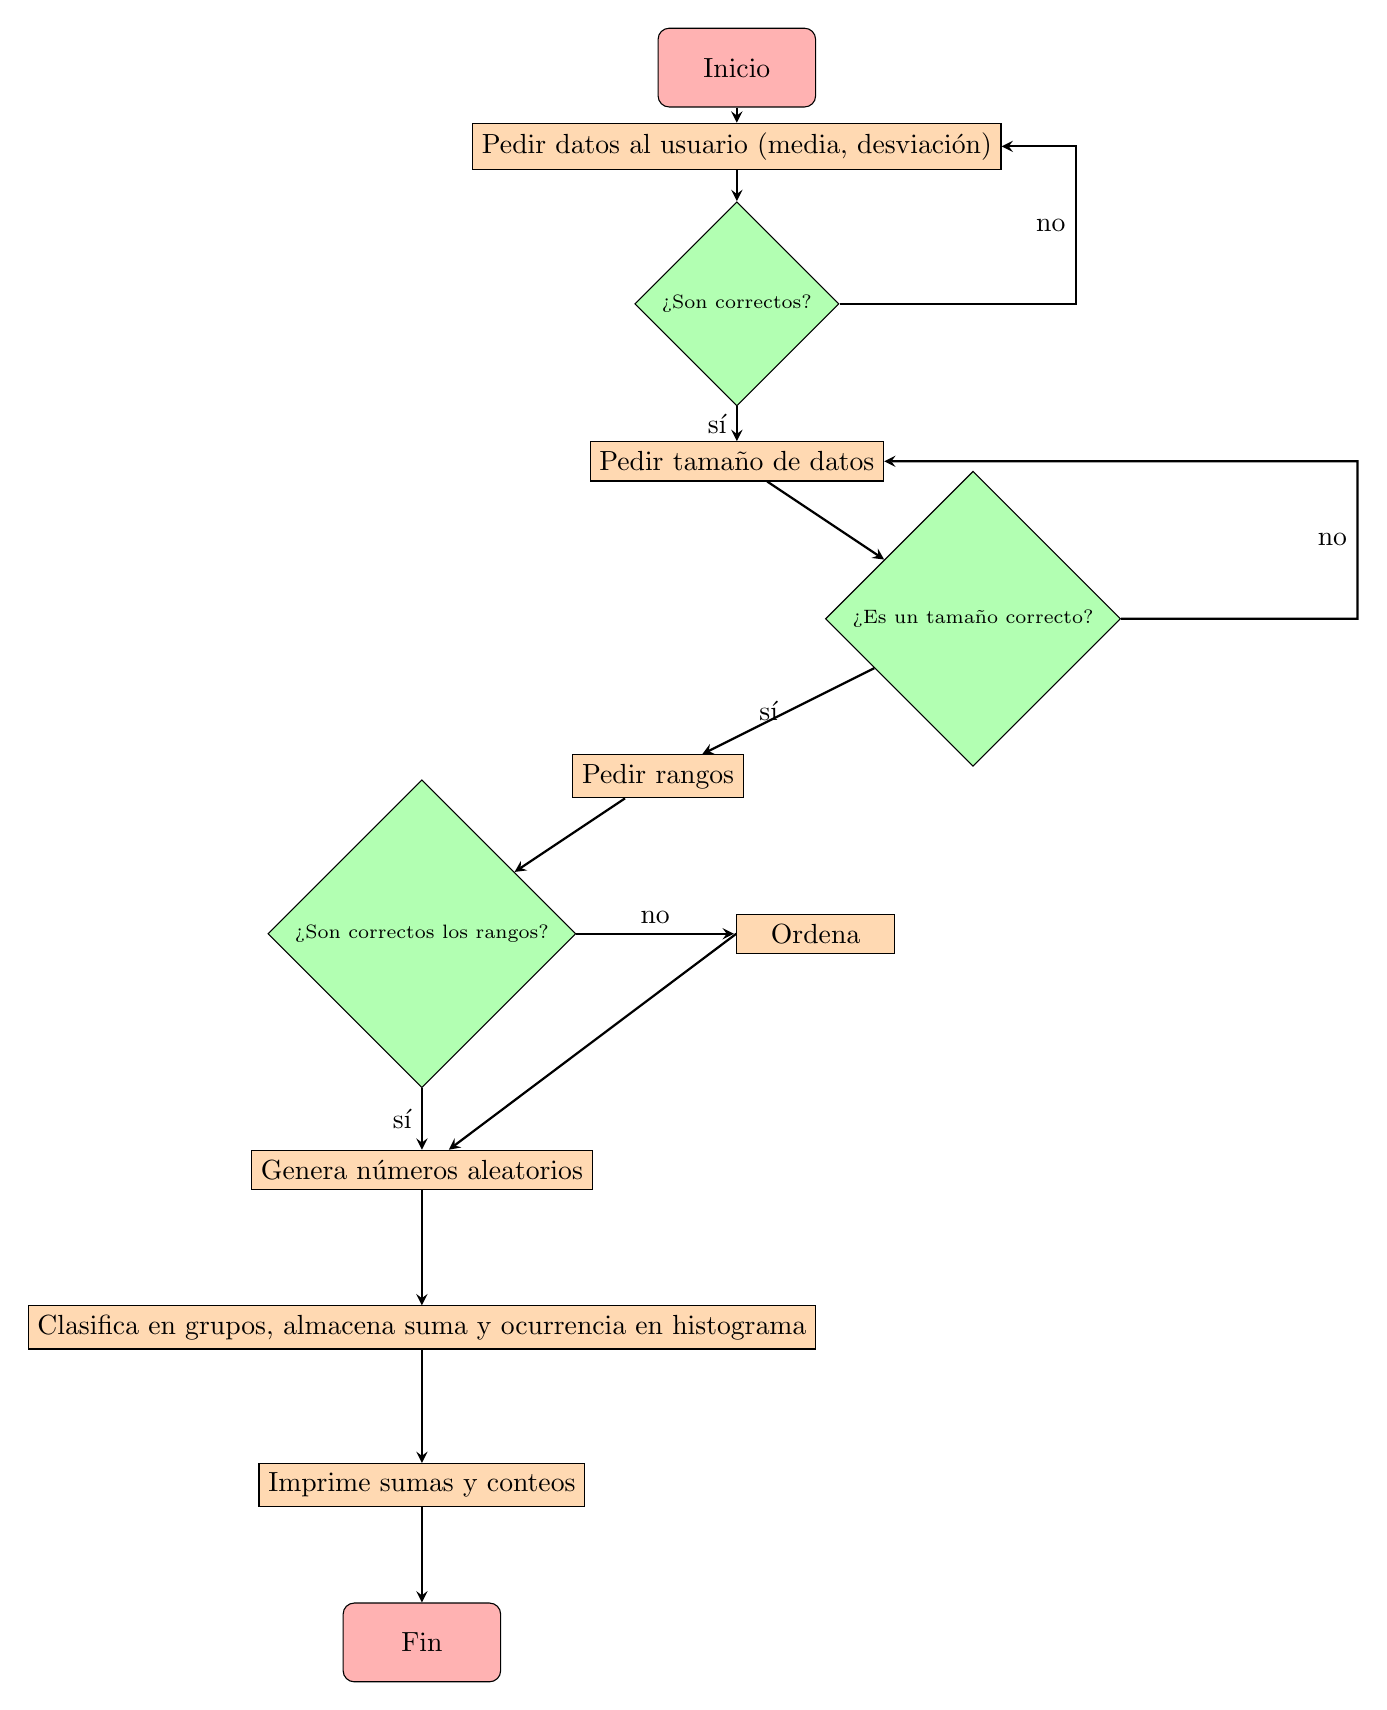
\begin{tikzpicture}[node distance=1cm]

    % Nodes
    \node (start) [startstop] {Inicio};
    \node (input) [process, below of=start] {Pedir datos al usuario (media, desviación)};
    \node (checkdata) [decision, below of=input, yshift=-1cm] {¿Son correctos?};
    \node (inputsize) [process, below of=checkdata, yshift=-1cm] {Pedir tamaño de datos};
    \node (checksize) [decision, right of=inputsize, yshift=-2cm, xshift=2cm]  {¿Es un tamaño correcto?};
    \node (inputrange) [process, left of=checksize, yshift=-2cm,xshift=-3cm] {Pedir rangos};
    \node (checkrange) [decision, left of=inputrange, yshift=-2cm,xshift=-2cm] {¿Son correctos los rangos?};
    \node (sort) [process, right of=checkrange, xshift=4cm] {Ordena};
    \node (generatenum) [process, below of=checkrange, yshift=-2cm] {Genera números aleatorios};
    \node (classify) [process, below of=generatenum, yshift=-1cm] {Clasifica en grupos, almacena suma y ocurrencia en histograma};
    \node (print) [process, below of=classify, yshift=-1cm] {Imprime sumas y conteos};
    \node (stop) [startstop, below of=print, yshift=-1cm] {Fin};
    
    % Arrows
    \draw [arrow] (start) -- (input);
    \draw [arrow] (input) -- (checkdata);
    \draw [arrow] (checkdata) -- node[anchor=east] {sí} (inputsize);
    \draw [arrow] (inputsize) -- (checksize);
    \draw [arrow] (checksize) -- node[anchor=east] {sí} (inputrange);
    \draw [arrow] (inputrange) -- (checkrange);
    \draw [arrow] (checkrange) -- node[anchor=east] {sí} (generatenum);
    \draw [arrow] (generatenum) -- (classify);
    \draw [arrow] (classify) -- (print);
    \draw [arrow] (print) -- (stop);
    
    % Loop for incorrect data
    \draw [arrow] (checkdata.east) -- ++(3,0) -- node[anchor=east] {no} ++(0,2) -- (input.east);
    \draw [arrow] (checksize.east) -- ++(3,0) -- node[anchor=east] {no} ++(0,2) --  (inputsize.east); 
    \draw [arrow] (checkrange.east) -- node[anchor=south] {no} ++(2,0) ; 
    \draw [arrow] (sort.west) --  (generatenum);
    \end{tikzpicture}
}
Se inicializa pidiendo datos de entrada, como son la media y desviación y se verifican si son correctos los datos ingresados, si no fue correcto se repite la pregunta, si fue correcto, entonces prosigue a preguntar la cantidad de piezas hasta que ingrese un tamaño adecuado. Se piden los intervalos, que si bien, siendo la ventaja del problema que solamente existen tres intervalos, de los cuales, solamente es necesario conocer dos valores, por lo que solamente sería necesario hacer un SWAP de división ya que estamos manejando números flotantes y tener la consideración de la existencia de algún 0 en cualquiera de los dos valores, debido a esto, ya que solo son condiciones y operaciones con complejidad constante, el SWAP posee una complejidad \(O(1)\). Si en dado caso, nuestro arreglo tuviera más intervalos, se tendrían que ordenar y uno de los mejores algoritmos de ordenamiento con respecto a su complejidad es el  \textit{Quick sort} que posee una complejidad algorítmica de $O(n\log(n))$, sin embargo, dado al problema a resolver, solo se limita a una complejidad constante.
Además de ello, también debe de verificar si en dado caso, los tiempos que ingreso no son menores a 0, si es así, vuelve a preguntar.
Después de ello, se generan los números aleatorios y se seleccionan acorde a si son procesos rápidos, normales o lentos.
Finalmente se imprimen las sumas de tiempos para cada intervalo y el tiempo total, adicionalmente el histograma de cuantas piezas se fabricaron con un proceso rápido, normal o lento.
\subsection{Diagrama de flujo}
\scalebox{0.8}{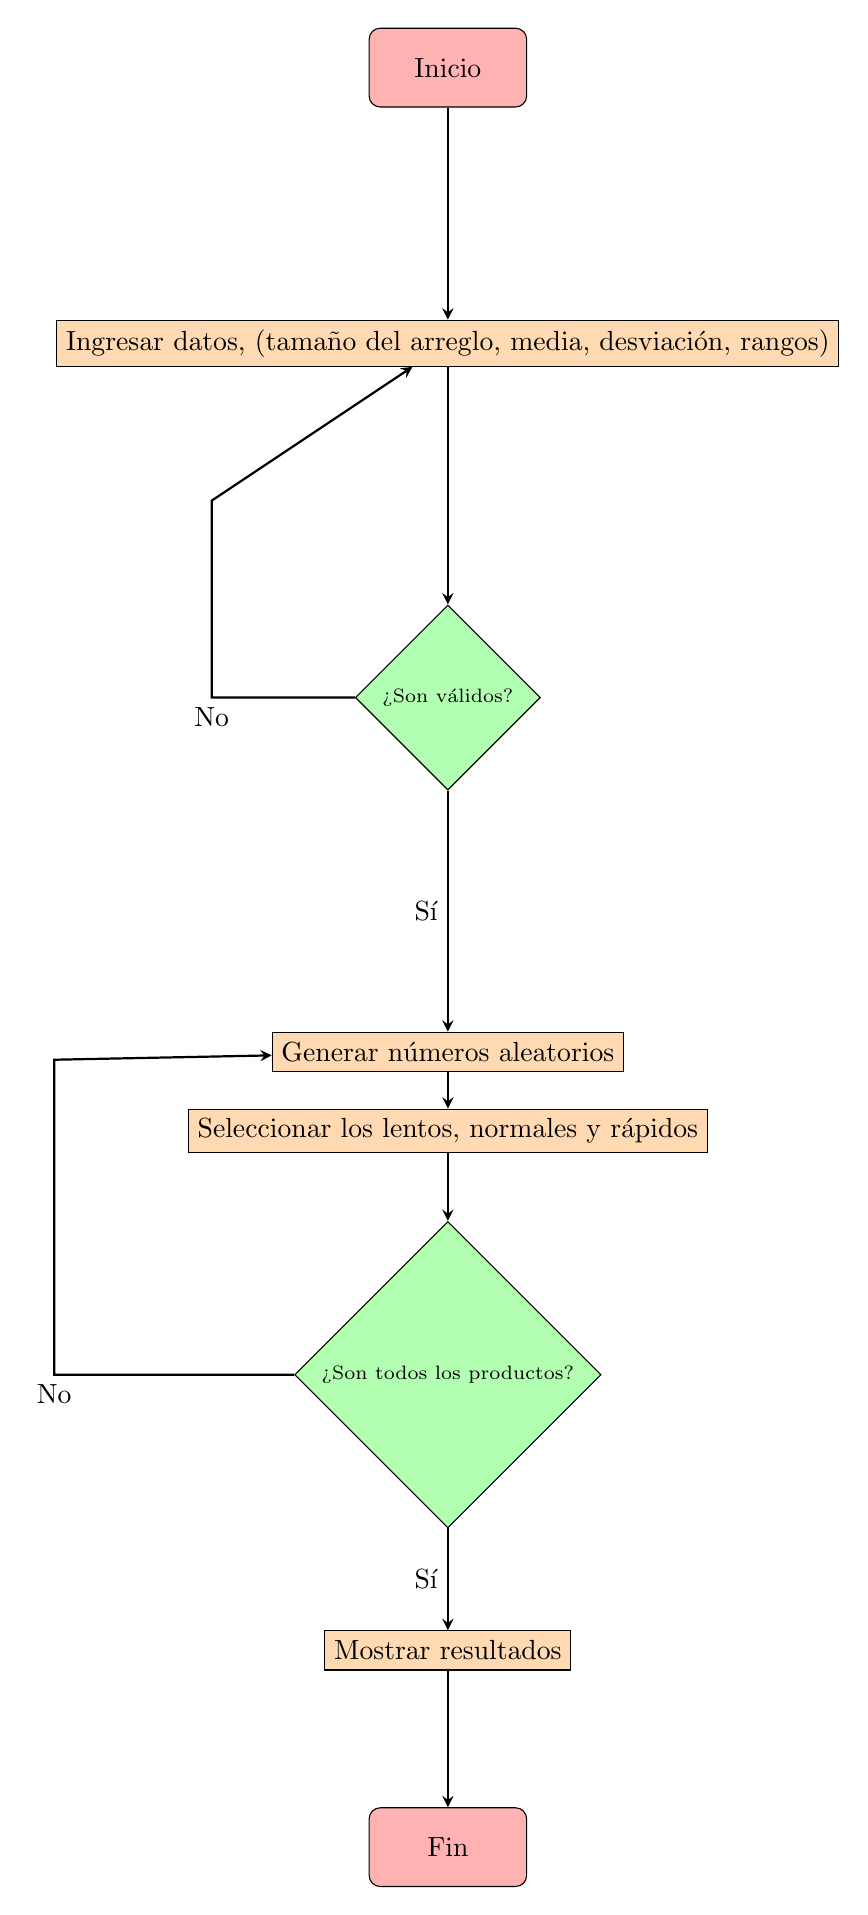
\begin{tikzpicture}[node distance=3cm] % Ajusta la distancia entre nodos a 3 cm

    \node (start) [startstop] {Inicio};
    \node (input) [process, below of=start, yshift=-0.5cm] {Ingresar datos, (tamaño del arreglo, media, desviación, rangos)};
    \node (check1) [decision, below of=input, yshift=-1.5cm] {¿Son válidos?};

  
    \node (loop) [process, below of=check1, yshift=-1.5cm] {Generar números aleatorios};
    
    \node (selection) [process, below of=loop, yshift=2cm] {Seleccionar los lentos, normales y rápidos};
    \node (check3) [decision, below of=selection, yshift=-0.1cm] {¿Son todos los productos?};

    \node (output) [process, below of=check3, yshift=-0.5cm] {Mostrar resultados};
    \node (stop) [startstop, below of=output, yshift=0.5cm] {Fin};
    
    % Flechas
    \draw [arrow] (start) -- (input);
    \draw [arrow] (input) -- (check1);
    \draw [arrow] (check1) -- node[anchor=east] {Sí} (loop);
    
  
  
    \draw [arrow] (loop) -- (selection);
    \draw [arrow] (selection) -- (check3);
    \draw [arrow] (output) -- (stop);
    \draw [arrow] (check1) -- ++(-3,0) node[anchor=north] {No} -- ++(0,2.5) -- (input);
    \draw [arrow] (check3) -- node[anchor=east] {Sí} (output);
    \draw [arrow] (check3) -- ++(-5,0) node[anchor=north] {No} -- ++(0,4) -- (loop);
    \end{tikzpicture}
    }
    El proceso para generar numeros aleatorios fue el siguiente

    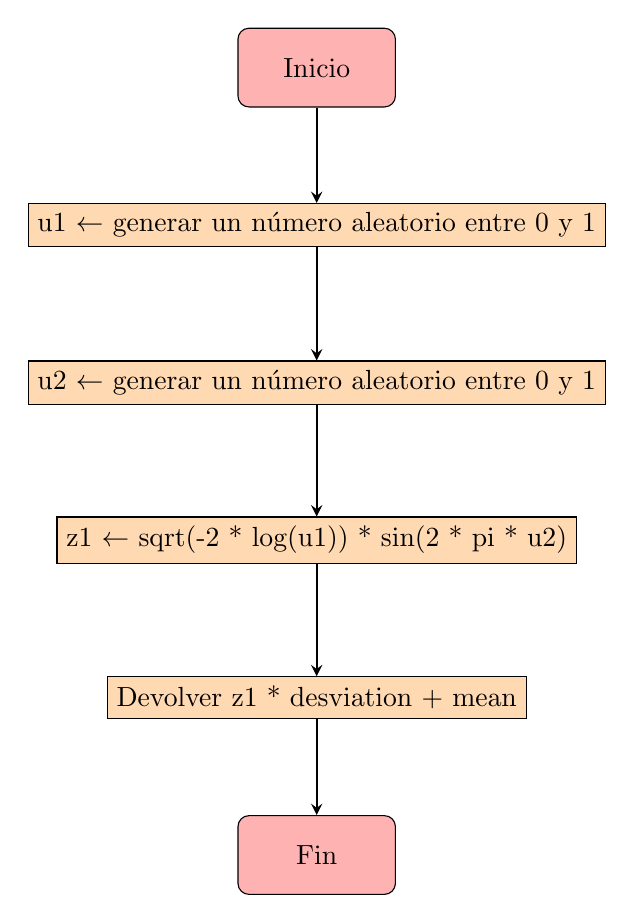
\begin{tikzpicture}[node distance=2cm]

        \node (start) [startstop] {Inicio};
        \node (input1) [process, below of=start] {u1 $\gets$ generar un número aleatorio entre 0 y 1};
        \node (input2) [process, below of=input1] {u2 $\gets$ generar un número aleatorio entre 0 y 1};
        \node (calc) [process, below of=input2] {z1 $\gets$ sqrt(-2 * log(u1)) * sin(2 * pi * u2)};
        \node (output) [process, below of=calc] {Devolver z1 * desviation + mean};
        \node (stop) [startstop, below of=output] {Fin};
    
        % Flechas
        \draw [arrow] (start) -- (input1);
        \draw [arrow] (input1) -- (input2);
        \draw [arrow] (input2) -- (calc);
        \draw [arrow] (calc) -- (output);
        \draw [arrow] (output) -- (stop);
    
    \end{tikzpicture}
    

    \subsection{Pseuodcódigo}
    \begin{algorithm}
        \caption{Proceso de generación y clasificación de productos}
        \begin{algorithmic}
        \STATE \textbf{Inicio}
        \STATE Ingresar datos (tamaño del arreglo, media, desviación, rangos)
        \IF{los datos son válidos}
            \STATE Generar números aleatorios
            \STATE Seleccionar los lentos, normales y rápidos
            \FOR{cada producto en el arreglo}
                \STATE Generar números aleatorios
                \STATE Seleccionar los lentos, normales y rápidos
            \ENDFOR
            \STATE Mostrar resultados
        \ELSE
            \STATE Volver a ingresar datos
        \ENDIF
        \STATE \textbf{Fin}
        \end{algorithmic}
    \end{algorithm}
La transformación de Box Müller es necesaria para poder transformar datos de una distribución uniforme a una distribución Gaussiana,siendo: 
$$Z_1=\sqrt{-2\ln(U_1)} \cdot \sin(2\cdot \pi \cdot U_2)$$
$$Z_0=\sqrt{-2\ln(U_1)} \cdot \cos(2\cdot \pi \cdot U_2)$$
$$X= z_1 \cdot \sigma+\mu$$
Siendo $U_1,U_2$ distribuciones uniformes continuas
Este es el proceso general con el que se diseño el algoritmo, sin embargo, el proceso para generar los números aleatorios es el siguiente:
\begin{algorithm}
    \caption{Función de normalización usando la transformación Box-Müller}
    \begin{algorithmic}[1] % [1] numera las líneas
        \STATE \textbf{Función} norm(mean, desviation)
        \STATE \(u1 \gets \text{generar un numero aleatorio entre 0 y 1}\)
        \STATE \(u2 \gets \text{generar un numero aleatorio entre 0 y 1}\)
        \STATE \(z1 \gets \sqrt{-2 \cdot \log(u1)} \cdot \sin(2 \cdot \pi \cdot u2)\)
        \STATE \textbf{devolver} $z1 \cdot desviation + mean$
        \STATE \textbf{Fin Función}
    \end{algorithmic}
\end{algorithm}

Para generar las clasificaciones existen diversos métodos:
\begin{itemize}
    \item If-ELSE
    \item Bitwise
    \item Relación logarítmica
    \item Sistemas de ecuaciones 
\end{itemize}
\subsection*{if-else}
La manera, if-else, solo sería con condiciones encadenadas de ifelse, siendo el primer caso, el número $d$ que se generó por la distribución, es menor a al primer rango, sino, se va a la siguiente condición en la que pregunta si es menor a el segundo rango y sino, se va el ultimo rango.
\subsection*{bitwise}
De esa manera se parte que tenemos dos condiciones y un indice que recorrer.
Se puede observar, que en un principio, las dos condiciones son verdaderas, después la primera condición es falsa, y finalmente ambas son falsas y al recorrer el indice de rangos que generamos, va de 0 a n-1, siendo n el número de rangos, por lo tanto, el arreglo tiene una longitud de 3.
\begin{table}[h]
    \centering
    \caption{Tabla de comparaciones en binario y decimal}
    \begin{tabular}{cccccc}
        \toprule
       value & \(c_1\) & \(c_0\) & \texttt{index} (Decimal) & \(b_1\) & \(b_0\) \\
        \midrule
    3 &   1       & 1       & 0                      & 0      & 0      \\
    1 &   0       & 1       & 1                      & 0      & 1      \\
    0 &   0       & 0       & 2                      & 1      & 0      \\
        \bottomrule
    \end{tabular}
\end{table}
Siendo $c_1=d<M[0] \text{  Siendo M, el arreglo de rangos}$, y $c_0=d<M[1]$ 
Por lo que se busca simplificar su forma lógica de tal forma que se utiliza un mapa de Karnaugh

\section*{Mapa de Karnaugh para \(b_1\)}
\[
\begin{array}{c|c|c}
c_1 \backslash c_0 & 0 & 1 \\
\hline
0 & 1 & 0 \\
1 & x & 0 \\
\end{array}
\]
Siendo su reducción como:
\begin{equation}
    b_1=c_1'c_0'
\end{equation}
\section*{Mapa de Karnaugh para \(b_0\)}
\[
\begin{array}{c|c|c}
c_1 \backslash c_0 & 0 & 1 \\
\hline
0 & 0 & 1 \\
1 & x & 0 \\
\end{array}
\]
La reducción de $b_0$
\begin{equation}
    b_0=c_1'c_0
\end{equation}
Resultando como la operación completa tal que:

\begin{align}
    b &= b_1 + b_0 \\
    b &= c_1'c_0' + c_1'c_0 \\
    b &= (\sim (d<M[0]) \cdot \sim (d<M[1])) + (\sim (d<M[0]) \cdot (d<M[1])) \\
    b &= ((d>M[0]) \cdot (d>M[1])) + ((d>M[0]) \cdot (d<M[1]))
\end{align}
Por lo que la Ecuación 8 terminaría siendo el valor que utilizaríamos para agregar a cada uno de los indices.
\subsection*{Logaritmo}
El método del logaritmo se calcula partiendo de la relación de los números de la tabla 1. Podemos observar que los valores van de 0,1,3,mientras que los indices van de 0 a 2. Se puede generar un modelo que siga la sucesión, de tal forma que
\begin{equation}
    2^{2-y}=x+1
\end{equation}
De esta manera, se puede calcular el recorrido del arreglo a través de la relación de concurrencia entre los datos de entrada y salida.
Lo que sería necesario saber sería calcular el valor de $y$, por el cuál, se ingresara en un switch y delimitará los valores que son de la sucesión.
\begin{align}
    \log_2(2^{2-y}) &= \log_2(x+1) \\
    (2-y)\log_2(2) &= \log_2(x+1) \\
    2 - y &= \log_2(x+1) \\
    y &= 2 - \log_2(x+1) \\
    y &= 2\log_2(2) - \log_2(x+1) \\
    y &= \log_2\left(\frac{2}{x+1}\right) \\
    y &= \frac{\ln\left(\frac{2}{x+1}\right)}{\ln(2)}
\end{align}
\subsection*{Polinomios}
El método de los polinomios se hace proponiendo un polinomio del grado de la cantidad de intervalos 

\begin{equation}
    y=a_2x^2+a_1x+a_0
\end{equation}

Después, se evalua con los valores de x y de y asociados
\begin{align}
    x=0,& y=3 \\
    3 &= a_0 \\
    x=1,& y=1 \\
    1&=a_2+a_1+3\\
    x=2 &, y=0 \\
    0 &=4a_2+2a_1+3
\end{align}
Se resuelve el sistema de ecuaciones para encontrar el valor de $a_0$ y $a_1$ con las ecuaciones 21 y 23
$$0=a_2+a_1+2$$
$$a_2=-a_1-2$$
Se sustituye en la ecuación 23
$$ 0=4(-a_1-2)+2a_1+3$$
$$0=-4a_1-8+2a-1+3$$
$$2a_1=-5$$
$$a_1=\frac{-5}{2}$$
Por lo tanto:
$$a_2=-(\frac{-5}{2})-2 \rightarrow a_2=\frac{5}{2}-2$$
$$a_2=\frac{1}{2}$$
Así que el polinomio de interés es 
\begin{equation}
    y=\frac{1}{2}x^2-\frac{5}{2}x+a_0
\end{equation}
\subsection{Flujo de información y sinergia de los datos}
El diagrama de la sección 3.2, a pesar de ser el que describe por completo el algoritmo, sirve como referencia para visualizar la sinergia de los datos, desde las peticiones y validaciones de datos, a su vez que al generar los números aleatorios, se requiere la media y la desviación de tal forma que genera números aleatorios, (sin embargo, lso números aleatorios generados por la función rand, son valores de una distribución uniforme), por lo que la transformación Box-Müller ayuda a pasar la distribución uniforma a gaussiana. Después,se agrupan los datos por algún método los valores calculados, (mencionados en la anterior sección). Finalmente se realizan las sumas,los histogramas y los promedios de cada valor.
\section{Resultados y análisis} Se hacen 6 experimentos de cada uno de 1000 productos y a su vez, con los rangos de 25,35 y con una $\mu=30$ y $\sigma=5$. Se encontró lo siguiente:
\subsection{Tablas de resultados con explicación}
\begin{table}[H]
    \centering
    \caption{Tabla comparativa 1}
    \begin{tabular}{cccccc}
        \toprule
       cálculos$\backslash $Procesos & rápidos & normales & lentos & totales \\
        \midrule
    sumas &   3560.73       & 19954.61       & 6574.46       & 30062.81           \\
    histogramas &   159       & 668       & 173          & 1000            \\
    medias &   22.39       & 29.87       & 37.84         & 30.06            \\
        \bottomrule
    \end{tabular}
\end{table}
\begin{table}[H]
    \centering
    \caption{Tabla comparativa 2}
    \begin{tabular}{cccccc}
        \toprule
       cálculos$\backslash$ Procesos & rápidos & normales & lentos & totales \\
        \midrule
    sumas &   3725.13       & 20089.18       & 6134.47       & 29948.80           \\
    histogramas &   166       & 671       & 163          & 1000            \\
    medias &   22.44       & 29.93       & 37.63         & 29.94            \\
        \bottomrule
    \end{tabular}
\end{table}
\begin{table}[H]
    \centering
    \caption{Tabla comparativa 3}
    \begin{tabular}{cccccc}
        \toprule
       cálculos$\backslash$ Procesos & rápidos & normales & lentos & totales \\
        \midrule
    sumas &   3817.29       & 20144.03       & 6154.59       & 30115.91           \\
    histogramas &   169       & 667       & 164          & 1000            \\
    medias &   22.58       & 30.20       & 37.52         & 30.11            \\
        \bottomrule
    \end{tabular}
\end{table}
\begin{table}[H]
    \centering
    \caption{Tabla comparativa 4}
    \begin{tabular}{cccccc}
        \toprule
       cálculos\ Procesos & rápidos & normales & lentos & totales \\
        \midrule
    sumas &   3557.40       & 20424.21       & 5832.93       & 29814.55           \\
    histogramas &   161       & 684       & 155          & 1000            \\
    medias &   22.09       & 29.85       & 37.63         & 30.11            \\
        \bottomrule
    \end{tabular}
\end{table}
\begin{table}[H]
    \centering
    \caption{Tabla comparativa 5}
    \begin{tabular}{cccccc}
        \toprule
       cálculos\ Procesos & rápidos & normales & lentos & totales \\
        \midrule
    sumas &   3961.75       & 19570.10       & 6390.39       & 29922.25           \\
    histogramas &   177       & 652       & 171          & 1000            \\
    medias &   22.38       & 30.01       & 37.37         & 29.92            \\
        \bottomrule
    \end{tabular}
\end{table}

\begin{table}[H]
    \centering
    \caption{Tabla comparativa 6}
    \begin{tabular}{cccccc}
        \toprule
       cálculos\ Procesos & rápidos & normales & lentos & totales \\
        \midrule
    sumas &   3494.83       & 20540.35       & 6015.70  & 20540.35           \\
    histogramas &   156       & 684       & 160          & 1000            \\
    medias &   22.40       & 30.02       & 37.59         & 30.05            \\
        \bottomrule
    \end{tabular}
\end{table}
Con respecto a los datos, se puede observar que la mayor cantidad de piezas se producen con un tiempo normal,las piezas rápidas y lentas en algunos experimentos suelen tener más que su contraparte o menos. Sin embargo, se puede observar que el tiempo medio de los valores normales por lo general suele ser de 30 minutos, mientras que los procesos rápidos es de 22.40 minutos y en los lentos es de 37.59 minutos
Tómese en cuenta, los datos fueron generados aleatoriamente, y los procesos que se realizaron con respecto al tiempo, pueden ser distintos en cada ordenador, sin embargo, independientemente de ese punto, los datos van a seguir la tendencia normal que observamos.
\subsection{Análisis de desempeño, precisión, eficiencia, repetibilidad y complejidad}
\subsection*{Análisis de desempeño temporal}
Si observamos y calculamos el tiempo a partir de que se procesan los datos, podemos observar que tarda 5 segundos, esto es debido el tiempo que pueda tomar al usuario capturar los elementos pedidos, sin embargo si se calcula solamente si tomamos en cuenta el tiempo en el que empieza a hacer los procesos, siendo 1000 elementos, 3 rangos de categorización, el tiempo es de 0.023 segundos aproximadamente.
\subsection*{Precision.}
El proceso que se hizo, no posee algún dato de referencia en el cual basarse su precisión, sin embargo, se puede tomar en cuenta la precisión de los valores flotantes y enteros. Para no tener problemas con respecto a las decimales, se toman solamente dos decimales. Sabiendo que las variables de tipo float por lo general poseen 4 bytes, si el número crece, las decimales cada vez se tornan más imprecisas, por lo que se toman solo dos decimales para el cálculo.
\subsection*{Repetibilidad}
Como se observó en la sección anterior, las tablas muestran la forma en como se desempeña el algoritmo. Se sabe que es un simulación que sigue una simulación basándose en el tiempo, por lo que los valores aleatorios generados difícilmente serán iguales. Sin embargo el resultado final que recopila los valores de las medias podemos observar que los valores siguen una misma tendencia de valores, la desviación se ve representada en que tan dispersos están los valores anteriores.
\subsection*{Complejidad}
El algoritmo base, presenta por lo general variables con una complejidad de $O(1)$, inclusive los rangos están definidos en un cierto intervalo, además, los valores de petición de se enmarcan hasta el valor 1000, sin está definición, el almacenamiento sería lineal con respecto a lo que el usuario vaa ingresando, sin embargo, se trunca hasta el valor 1000.

Observe también la complejidad temporal, la petición de los datos del usuario terminan siendo constantes en su mayoría, ya que solamente se piden una vez y se validan los datos.
El procesamiento de los datos es lo que hace que varié, y en este caso, dado a que tenemos nuestra memoria lineal donde está la cantidad de datos. Por lo que el proceso de añadir los es lineal $O(n)$. 
Sin embargo, el método de selección de variables puede que haga más complejo el problema.
Principalmente, la librería math puede que utilice un proceso con complejidad $O(n)$ para calcular el logaritmo natural y la función seno, dado a que suele utilizar las series de Taylor como método numérico para poder  calcular las funciones. Sin embargo al estar anidado dentro del bucle que recorre el arreglo hace que el algoritmo esté dado por una complejidad de $O(n^n)$ sin embargo, las funciones calculadas por la serie de Taylor están dadas por el tiempo, así que el valor podría ser lo suficiente pequeño de tal modo que el algoritmo quede como $O(n)$. 
Sabemos que existen 4 métodos posibles para determinar los rangos, el método if/else siendo uno de los más intuitivos y legibles posibles para ser implementado. El método BitWise funge como un if, sin embargo, debido a que son operaciones binarias, al CPU le resulta más fácil calcularlo, a pesar de que la parte del ALU de un procesador se encuentre los procesamientos lógico/aritméticos, los valores lógicos le resultan más fácil de calcularlos. Sin embargo el problema que posee BitWise es que solamente se limita al rango ya definido. Si queremos dinamismo, puede ser da gran utilidad o usar la forma polinomial de seleccionar los datos y la logarítmica. Ya que con la forma polinomial se puede generar un algoritmo Gauss-Jordan que calcule cada valor de los coeficientes del polinomio y si se ingresan los rangos de forma dinámica, lo que haría sería calcular dinámicamente los valores, aunque si bien, el problema se podría visualizar, que cada que vez que se compila, haría más lento el cálculo debido a que crecería la complejidad del problema y su memoria necesaria para procesar el algoritmo.
De igual forma, la metodología por logaritmo, a pesar de que puede resultar efectivo si la cantidad de rangos es dinámico pasaría algo similar con respecto al peso algoritmo de calcular un logaritmo.

Si se mantiene estático el valor de los parámetros, el método podría ser útil ya que no es necesario generar un algoritmo que calcule lo valores de los coeficientes, además de que las operaciones se producen en tiempo de $O(1)$.
\section{Tabla comparativa}
Se debe tomar con mucha cautela el valor proporcionado del tiempo, ya que el tiempo de proceso puedo ser distinto entre máquinas que tengan cierto tipo de procesadores, por lo que la velocidad de procesamiento con respecto a un i9 y a un i7 de la familia Intel, arrojará diferentes resultados.
Lo importante a tomar en cuenta sería comparar la complejidad del procesamiento. De esta manera, podemos aplicarlo en diferentes ordenadores.
Se proponen 4 modelos, polinomial, logarimtico, por BitWise y por if-switch
\subsection{Análisis de eficiencia y desempeño}

\begin{table}[h!]
    \centering
    \begin{tabular}{@{}lcccc@{}}
        \toprule
        \textbf{Método} & \textbf{Complejidad} & \textbf{Rendimiento} & \textbf{Legibilidad}  \\ \midrule
        \textbf{Bitwise} & \( O(1) \) & Muy alto & Medio  \\
        \textbf{`if-else` / `switch-case`} & \( O(1) \) & Alto & Muy alto  \\
        \textbf{Logaritmo Natural} & \( O(1) \) & Medio & Medio \\
        \textbf{Polinomial} & \( O(1) \) & Medio & Medio  \\ \bottomrule
    \end{tabular}
    \caption{Comparación de Métodos de Clasificación}
\end{table}
El calculo de logaritmo natural por parte de la librería ha sido optimizado de tal forma, que pueda ser considerado complejidad. Como se había mencionado anteriormente, en algunos casos puede que la complejidad de los cálculos de funciones matemáticas por parte de la biblioteca puede ser considerado lineal o en el mejor caso constante. 
Sin embargo, como se puede ver mediante la tabla, BitWise posee un mayor rendimiento debido a que son operaciones binarias, mientras que if/else posee un rendimiento alto, no demasiado como bitwise, sin embargo es un código más legible el utilizar if/else o switch.
Por su parte, el logaritmo natural es un poco más costoso de utilizar al igual que el polinomio, y a pesar de que los valores definidos por el problema permite que estas operaciones sean constantes, la complejidad aumenta. 
\subsection{Comparativa con el estado del arte}
Para el articulo \citep{article}muestra de manera simplifica el cómo el método BitWise puede ayudar a reducir la complejidad del código, siendo que muchas condiciones de if/else, se reducen a valores binarios que pueden ser representados como tal, haciendo que el proceso sea mucha más rápido, además \citep{chandra2013application}, menciona más ejemplos de uso y sobre todo, muestra la manera en la que operaciones aritméticas también pueden ser reducidas.
BitWise es una metodología eficiente, sin embargo, en este código, los cambios no vana ser notorios debido a la pequeña cantidad de datos existentes.
\section{Conclusiones}
Después de haber analizado tanto la eficiencia del algoritmo y de la selección de los objetos por tiempo de fabricación, a su vez como la inferencia de los resultados obtenidos de la simulación. La fábrica tendrá más procesos de tiempos normales, la cantidad de tiempos rápidos y lentos posee una pequeña diferencia de 2 unidades, siendo los tiempos rápidos el rango con esa ligera ventaja con respecto a los lentos. Dado a que es una distribución normal, estos valores van a seguir la tendencia y el sesgo que exista sería muy pequeño en comparación a otro tipo de distribuciones. 
Los métodos de selección de categorías pueden ser escogidos dado a la necesidad del problema, sin embargo los más habituales son los casos de if/else y BitWise. 
\bibliographystyle{apalike}
\bibliography{references.bib}
%\bibliography{}
\end{document}
